\chapter{Casos de uso extendidos}
\label{chap:CasosDeUsoExt}
En esta ap\'endice se proceder\'a a detallar cada caso de uso, dar una descripci\'on
de que se hace, que actores toman parte, precondiciones, requisitos no funcionales, el flujo de
eventos, as\'i como sus poscondiciones.

De esta manera se podr\'a comprender m\'as f\'acilmente el funcionamiento del software
sin la necesidad de utilizar el software o mirar el c\'odigo fuente e interfaz gr\'afica,
que se encuentra al final de este anexo.

Tambi\'en pongo aqu\'i el diagrama de casos de uso para que no haga falta
volver al cap\'itulo de Captura de requisitos.

\begin{figure}[h]
	\centering
	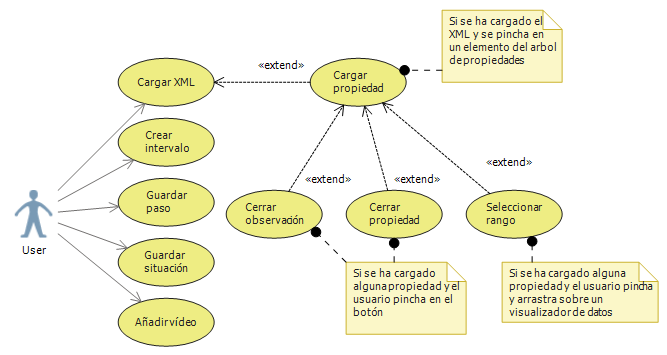
\includegraphics[width=0.7\linewidth]{./Figures/useCaseDiagram.png}
	\caption[Diagrama de casos de uso]{Diagrama de casos de uso}
\end{figure}

\section{Cargar XML}

\begin{table}[H]
	\begin{center}
		\rowcolors{2}{lightgray}{} %\rowcolors{<starting row index>}{<odd row color>}{<even row color>}
		\begin{tabular}{|l*{1}{p{10cm}}|}
			
			\multicolumn{2}{c}{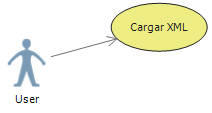
\includegraphics[width=0.36\linewidth]{./Figures/CargarXML.png}} \\
			\hline
		    Nombre                     & Cargar XML \\
		    Descripci\'on              & Carga un XML que contiene las propiedades
		    							 y las observaciones en el sistema. \'Unicamente
		    							 se cargan si el archivo valida contra el XSD.  \\ 
		    Actores                    & User  \\
		    Precondiciones             & Ninguna  \\
		    Requisitos no funcionales  & Ninguno  \\
		    Flujo de eventos           & \begin{enumerate}
		    								\item El usuario pincha en File -> Load XML.
		    								\item Se abre una ventana de selecci\'on de archivos.
		    								\item \textbf{Si el usuario quiere cargar un fichero}
		    								\begin{enumerate}
		    									\item Lo busca en el sistema de archivos [\ref{fig:AbrirXML1}]
		    									\item Lo selecciona y pincha en Abrir.
		    									\item \textbf{Si es un documento v\'alido}
		    									\begin{enumerate}
		    										\item Las observaciones y sus propiedades 
		    											  aparecen en el \'arbol lateral.
		    											  [\ref{fig:AbrirXML2}]
		    									\end{enumerate}
		    									\item \textbf{Si no}
		    									\begin{enumerate}
		    										\item Se muestra un error.
		    										[\ref{fig:AbrirXML3}]
		    									\end{enumerate}
		    								\end{enumerate}
		    								\item \textbf{Si no desea cargarlo}
		    								\begin{enumerate}
		    									\item Pincha en cancelar y se muestra un mensaje de que debe cargar un XML [\ref{fig:AbrirXML4}].
		    								\end{enumerate}
		    							 \end{enumerate} \\
		    Poscondiciones			   & El \'arbol contendr\'a las observaciones y 
		    							 propiedades si era un documento v\'alido, mostrar\'a
		    							 un error si era un documento inv\'alido, o mostrar\'a un aviso
                                         indicando de que se necesita cargar un XML para poder trabajar.  \\
		    Interfaz gr\'afica		   & Figuras \ref{fig:AbrirXML1}, \ref{fig:AbrirXML2},
		    							 \ref{fig:AbrirXML3} y \ref{fig:AbrirXML4}\\
		    \hline
		\end{tabular}
	\caption[Cargar XML]{Cargar XML}
	\label{Cargar XML}
	\end{center}
\end{table}

\section{A\~nadir v\'ideo}
\begin{table}[H]
	\begin{center}
		\rowcolors{2}{lightgray}{} %\rowcolors{<starting row index>}{<odd row color>}{<even row color>}
		\begin{tabular}{|l*{1}{p{10cm}}|}
			\multicolumn{2}{c}{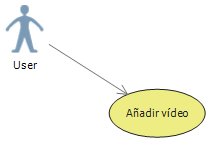
\includegraphics[width=0.4\linewidth]{./Figures/AnadirVideo.png}} \\
			\hline
		    Nombre                     & A\~nadir v\'ideo \\
		    Descripci\'on              & Abre un v\'ideo y lo a\~nade al contenedor
		    							 de v\'ideos si ya hab\'ia v\'ideos previamente
		    							 cargados. Si no, a\~nade tambi\'en un contenedor
		    							 de v\'ideos.  \\ 
		    Actores                    & User  \\
		    Precondiciones             & Ninguna  \\
		    Requisitos no funcionales  & Ninguno  \\
		    Flujo de eventos           & \begin{enumerate}
		    								\item El usuario pincha en Add Video.
		    								[\ref{fig:CargarVideo}]
		    								\item \textbf{Si el contenedor no de v\'ideos estaba
		    										      cargado}
	    									\begin{enumerate}
	    										\item Se crea y a\~nade un contenedor de v\'ideos.
	    									\end{enumerate}
	    									\item Se abre una ventana de selecci\'on de archivos.
		    								\item \textbf{Si el usuario quiere cargar v\'ideos}
		    								\begin{enumerate}
		    									\item Los busca en el sistema de archivos
		    									\item Los selecciona y pincha en Abrir.
		    									\item Se cargan si no estaban previamente cargados.
		    								\end{enumerate}
		    								\item \textbf{Si no desea cargarlo}
		    								\begin{enumerate}
		    									\item Pincha en cancelar.
		    								\end{enumerate}
		    							 \end{enumerate} \\
		    Poscondiciones			   & El contenedor con los nuevos v\'ideos a\~nadidos  \\
		    Interfaz gr\'afica		   & Figuras \ref{fig:CargarVideo}\\
		    \hline 
		\end{tabular}
	\caption[A\~nadir v\'ideo]{A\~nadir v\'ideo}
	\label{Anadir video}
	\end{center}
\end{table}

\section{Cargar propiedad}
\begin{table}[H]
	\begin{center}
		\rowcolors{2}{lightgray}{} %\rowcolors{<starting row index>}{<odd row color>}{<even row color>}
		\begin{tabular}{|l*{1}{p{10cm}}|}
			
			\multicolumn{2}{c}{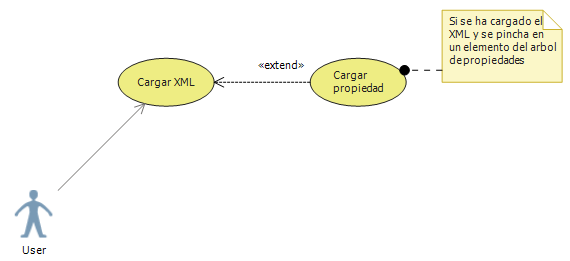
\includegraphics[width=0.6\linewidth]{./Figures/CargarPropiedad.png}} \\
			\hline
		    Nombre                     & Cargar propiedad \\
		    Descripci\'on              & Carga una propiedad en el contenedor de gr\'aficos
		    							 correspondiente a la observaci\'on a la que pertenece.
		    							 Tambi\'en puede a\~nadir propiedades en grupo, haciendo
		    							 doble click sobre el nombre de la observaci\'on. Si
		    							 el contenedor no est\'a creado, lo crea.  \\ 
		    Actores                    & User.  \\
		    Precondiciones             & Ninguna.  \\
		    Requisitos no funcionales  & Ninguno.  \\
		    Flujo de eventos           & \begin{enumerate}
		    								\item El usuario hace doble click en alg\'un elemento
		    									  del \'arbol de observaciones y propiedades.
		    								\item \textbf{Si el elemento es una observaci\'on}
		    								\begin{enumerate}
		    									\item Carga el contenedor si no estaba creado
		    									\item A\~nade todos sus hijos no cargados al
		    										  contenedor.
		    								\end{enumerate}
		    								\item \textbf{Si el elemento es una propiedad}
		    								\begin{enumerate}
			    								\item Crea el contenedor de la observaci\'on
			    									  a la que pertenece la propiedad seleccionada
			    									  si no estaba cargado.
			    								\item A\~nade la propiedad si no estaba cargada
			    									  previamente.
			    									  
		    								\end{enumerate}
		    							 \end{enumerate} \\
		    Poscondiciones			   & El contenedor de la observaci\'on y todas las 
		    							 propiedades de la observaci\'on o la propiedad
		    							 seleccionada dependiendo de d\'onde se haya hecho 
		    							 doble click y sincronizada con el rango existente, si es que lo hay. \\
		    Interfaz gr\'afica		   & Figuras \ref{fig:CargarObservacionPropiedad}\\
		    \hline
		\end{tabular}
	\caption[Cargar propiedad]{Cargar propiedad}
	\label{Cargar propiedad}
	\end{center}
\end{table}


\section{Seleccionar rango}

\begin{table}[H]
	\begin{center}
		\rowcolors{2}{lightgray}{} %\rowcolors{<starting row index>}{<odd row color>}{<even row color>}
		\begin{tabular}{|l*{1}{p{10cm}}|}
			
			\multicolumn{2}{c}{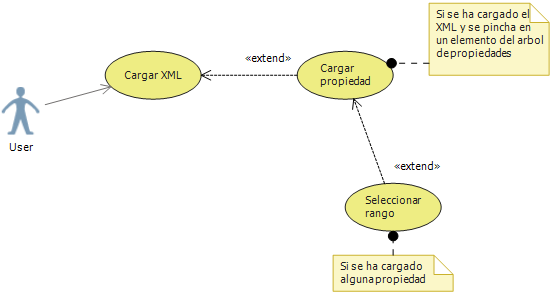
\includegraphics[width=1.0\linewidth]{./Figures/SeleccionarRango.png}} \\
			\hline
		    Nombre                     & Seleccionar rango \\
		    Descripci\'on              & Al pinchar y mover el rat\'on sobre un visualizador de datos,
		    							 se seleccionar\'a un rango en todos los visualizadores de datos
		    							 cargados en el sistema. \\ 
		    Actores                    & User  \\
		    Precondiciones             & Alguna propiedad tiene que estar cargada.  \\
		    Requisitos no funcionales  & Ninguno  \\
		    Flujo de eventos           & \begin{enumerate}
		    								\item El usuario pincha en un visualizador de datos.
		    								\item El usuario arrastra (manteniendo pinchado) el rat\'on.
		    								\begin{enumerate}
		    									\item Cada vez que el rango seleccionado cambia, se notifica al contenedor padre.
		    									\item El contenedor, notifica al repositorio de contenedores, para que todos
		    									se sincronicen con el dato proporciado.
		    									\item Se recorren todos los visualizadores de datos para sincronizarse con el nuevo
		    									valor.
		    								\end{enumerate}
		    								\item El usuario deja de pinchar, y se queda el rango seleccionado.
		    							 \end{enumerate} \\
		    Poscondiciones			   & El rango quedar\'a seleccionado en todos los 
		    							 visualizadores de datos
		    							 cargados en el sistema.  \\
		    Interfaz gr\'afica		   & Figuras \ref{fig:SeleccionarRango}\\
		    \hline
		\end{tabular}
	\caption[Seleccionar rango]{Seleccionar rango}
	\label{SeleccionarRango}
	\end{center}
\end{table}


\section{Cerrar observaci\'on}
\begin{table}[H]
	\begin{center}
		\rowcolors{2}{lightgray}{} %\rowcolors{<starting row index>}{<odd row color>}{<even row color>}
		\begin{tabular}{|l*{1}{p{10cm}}|}
			
			\multicolumn{2}{c}{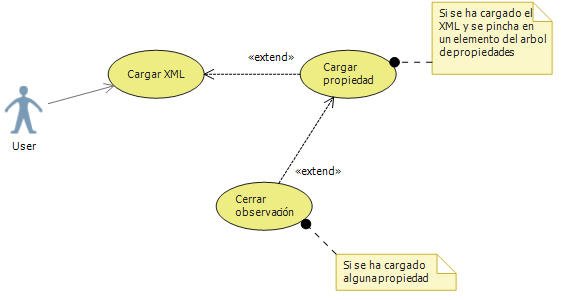
\includegraphics[width=1.0\linewidth]{./Figures/CerrarObservacion.png}} \\
			\hline
		    Nombre                     & Cerrar observaci\'on \\
		    Descripci\'on              & Elimina, tanto de manera visual, como de memoria, la observaci\'on
		    							 seleccionada y todos sus visualizadores de datos (propiedades) asociadas.  \\ 
		    Actores                    & User.  \\
		    Precondiciones             & La observaci\'on ten\'ia que estar cargada. \\
		    Requisitos no funcionales  & Ninguno.  \\
		    Flujo de eventos           & \begin{enumerate}
		    								\item El usuario pincha sobre la ``X" \ en la esquina
		    									  superior derecha de la observaci\'on.
		    								\item Se borra del repositorio, liberando sus recursos, y con ello,
		    									  sus propiedades.
		    								\item Finalmente se borra de la pantalla.
		    							 \end{enumerate} \\
		    Poscondiciones			   & El espacio de trabajo contendr\'a todas las observaciones
		    							 y propiedades menos la que se ha cerrado.  \\
		    Interfaz gr\'afica		   & Ninguna relevante.\\
		    \hline
		\end{tabular}
	\caption[Cerrar observaci\'on]{Cerrar observaci\'on}
	\label{Cerrar observacion}
	\end{center}
\end{table}


\section{Cerrar propiedad}
\begin{table}[H]
	\begin{center}
		\rowcolors{2}{lightgray}{} %\rowcolors{<starting row index>}{<odd row color>}{<even row color>}
		\begin{tabular}{|l*{1}{p{10cm}}|}
			
			\multicolumn{2}{c}{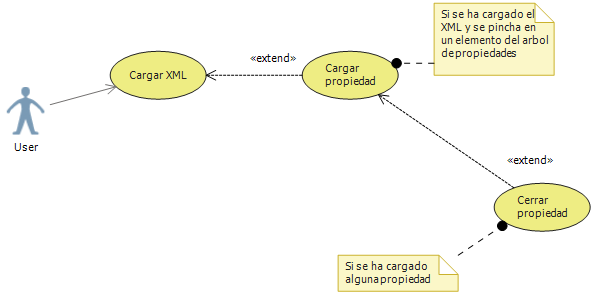
\includegraphics[width=1.0\linewidth]{./Figures/CerrarPropiedad.png}} \\
			\hline
			Nombre                     & Cerrar propiedad \\
			Descripci\'on              & Elimina, tanto de manera visual, como de memoria, la propiedad
									  	 seleccionada.  \\ 
			Actores                    & User.  \\
			Precondiciones             & La propiedad ten\'ia que estar cargada. \\
			Requisitos no funcionales  & Ninguno.  \\
			Flujo de eventos           & \begin{enumerate}
										 	\item El usuario pincha sobre la ``X" \ en la esquina
												  superior derecha de la propiedad.
											\item Se borra del contenedor al que estaba asociada.
											\item Finalmente se borra de la pantalla.
										 \end{enumerate} \\
			Poscondiciones			   & El espacio de trabajo contendr\'a todas las observaciones
										 y propiedades menos la propiedad que se ha cerrado.  \\
			Interfaz gr\'afica		   & Ninguna relevante\\
			\hline
		\end{tabular}
	\caption[Cerrar propiedad]{Cerrar propiedad}
	\label{Cerrar propiedad}
	\end{center}
\end{table}

\section{Crear intervalo}
\begin{table}[H]
	\begin{center}
		\rowcolors{2}{lightgray}{} %\rowcolors{<starting row index>}{<odd row color>}{<even row color>}
		\begin{tabular}{|l*{1}{p{10cm}}|}
			
			\multicolumn{2}{c}{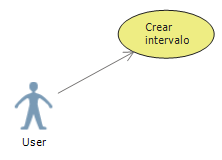
\includegraphics[width=0.4\linewidth]{./Figures/CrearIntervalo.png}} \\
			\hline
		    Nombre                     & Crear intervalo \\
		    Descripci\'on              & A\~nade el intervalo seleccionado
		    							 a los intervalos a guardar en el xml si
		    							 no se superpone con los que ya est\'an guardados.\\ 
		    Actores                    & User  \\
		    Precondiciones             & Alguna propiedad debe estar seleccionada
		    							 y un rango debe estar seleccionado.  \\
		    Requisitos no funcionales  & Ninguno  \\
		    Flujo de eventos           & \begin{enumerate}
		    								\item El usuario pincha Create interval.
		    								\item \textbf{Si el intervalo actual
		    								no se superpone con ninguno
		    								guardado previamente}
		    								\begin{enumerate}
		    									\item Se guarda el intervalo en la lista
		    									de intervalos a exportar.
		    									\item Se muestra un dialogo notificando que
		    									la operaci\'on se ha realizado correctamente. [\ref{fig:CrearIntervalo}]
		    								\end{enumerate}
		    								\item \textbf{Si se superpone}
		    								\begin{enumerate}
			    								\item Se muestra un dialogo notificando que
		    									el rango seleccionado se superpone con alguno
		    									guardado. [\ref{fig:CrearIntervaloError}]
		    								\end{enumerate}
		    								
		    							 \end{enumerate} \\
		    Poscondiciones			   & Se guardar\'a el nuevo intervalo en
		    							 lista de intervalos a exportar.  \\
		    Interfaz gr\'afica		   & Figuras \ref{fig:CrearIntervalo} y 
		    							 \ref{fig:CrearIntervaloError}\\
		    \hline
		\end{tabular}
	\caption[Crear intervalo]{Crear intervalo}
	\label{Crear Intervalo}
	\end{center}
\end{table}


\section{Guardar paso}
\begin{table}[H]
	\begin{center}
		\rowcolors{2}{lightgray}{} %\rowcolors{<starting row index>}{<odd row color>}{<even row color>}
		\begin{tabular}{|l*{1}{p{10cm}}|}
			
			\multicolumn{2}{c}{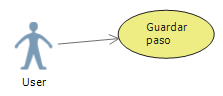
\includegraphics[width=0.4\linewidth]{./Figures/GuardarPaso.png}} \\
			\hline
		    Nombre                     & Guardar Paso. \\
		    Descripci\'on              & Guarda todos los intervalos creados
		    							 a disco con un elemento ra\'iz ``step".\\ 
		    Actores                    & User  \\
		    Precondiciones             & Ninguna.  \\
		    Requisitos no funcionales  & Ninguno  \\
		    Flujo de eventos           & \begin{enumerate}
		    								\item El usuario pincha en Save selected range -> Step. [\ref{fig:GuardarPaso1}]
		    								\item Se muestra un di\'alogo de guardado de datos.
		    								\item \textbf{Si el usuario decide guardar
		    								el fichero.}
		    								\begin{enumerate}
		    									\item Elige un nombre de fichero y pincha
		    									en guardar. [\ref{fig:GuardarPaso2}]
		    									\item El fichero se guarda en la carpeta
		    									especificada.
		    									\item Se borran todos los intervalos
		    									guardados.
		    								\end{enumerate}
		    								\item \textbf{Si pincha en cancelar}
		    								\begin{enumerate}
		    									\item Se cierra la ventana y no se borran
		    									los intervalos, para poder seguir trabajando.
		    								\end{enumerate}
		    								
		    							 \end{enumerate} \\
		    Poscondiciones			   & El fichero guardado en disco, o no,
		    						     dependiendo de las acciones del usuario.  \\
		    Interfaz gr\'afica		   & Figuras \ref{fig:GuardarPaso1} y \ref{fig:GuardarPaso2}\\
		    \hline
		\end{tabular}
	\caption[Guardar paso]{Guardar paso}
	\label{Guardar paso}
	\end{center}
\end{table}


\section{Guardar situaci\'on}
\begin{table}[H]
	\begin{center}
		\rowcolors{2}{lightgray}{} %\rowcolors{<starting row index>}{<odd row color>}{<even row color>}
		\begin{tabular}{|l*{1}{p{10cm}}|}
			
			\multicolumn{2}{c}{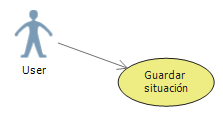
\includegraphics[width=0.4\linewidth]{./Figures/GuardarSituacion.png}} \\
			\hline
		    Nombre                     & Guardar situaci\'on \\
		    Descripci\'on              & Guarda todos los intervalos creados
  		    							 a disco con un elemento ra\'iz ``situation".\\ 
		    Actores                    & User  \\
		    Precondiciones             & Ninguna.  \\
		    Requisitos no funcionales  & Ninguno  \\
		    Flujo de eventos           & \begin{enumerate}
		    								\item El usuario pincha Save selected range -> 
		    								Situation. [\ref{fig:GuardarSituacion1}]
		    								\item Se muestra un di\'alogo de guardado de datos.
		    								\item \textbf{Si el usuario decide guardar
		    								el fichero.}
		    								\begin{enumerate}
		    									\item Elige un nombre de fichero y pincha
		    									en guardar. [\ref{fig:GuardarSituacion2}]
		    									\item El fichero se guarda en la carpeta
		    									especificada.
		    									\item Se borran todos los intervalos
		    									guardados.
		    								\end{enumerate}
		    								\item \textbf{Si pincha en cancelar}
		    								\begin{enumerate}
		    									\item Se cierra la ventana y no se borran
		    									los intervalos, para poder seguir trabajando.
		    								\end{enumerate}
		    								
										\end{enumerate} \\
			Poscondiciones			   & El fichero guardado en disco, o no,
										 dependiendo de las acciones del usuario.  \\
		    Interfaz gr\'afica		   & Figuras \ref{fig:GuardarSituacion1} y 
		    							 \ref{fig:GuardarSituacion2}\\
		    \hline
		\end{tabular}
	\caption[Guardar situaci\'on]{Guardar situaci\'on}
	\label{Guardar situacion}
	\end{center}
\end{table}

\pagebreak

\section{Figuras de los casos de uso}
Todas las figuras asociadas a los casos de uso extendidos pueden encontrarse en esta secci\'on

\begin{figure}[h]
\centering
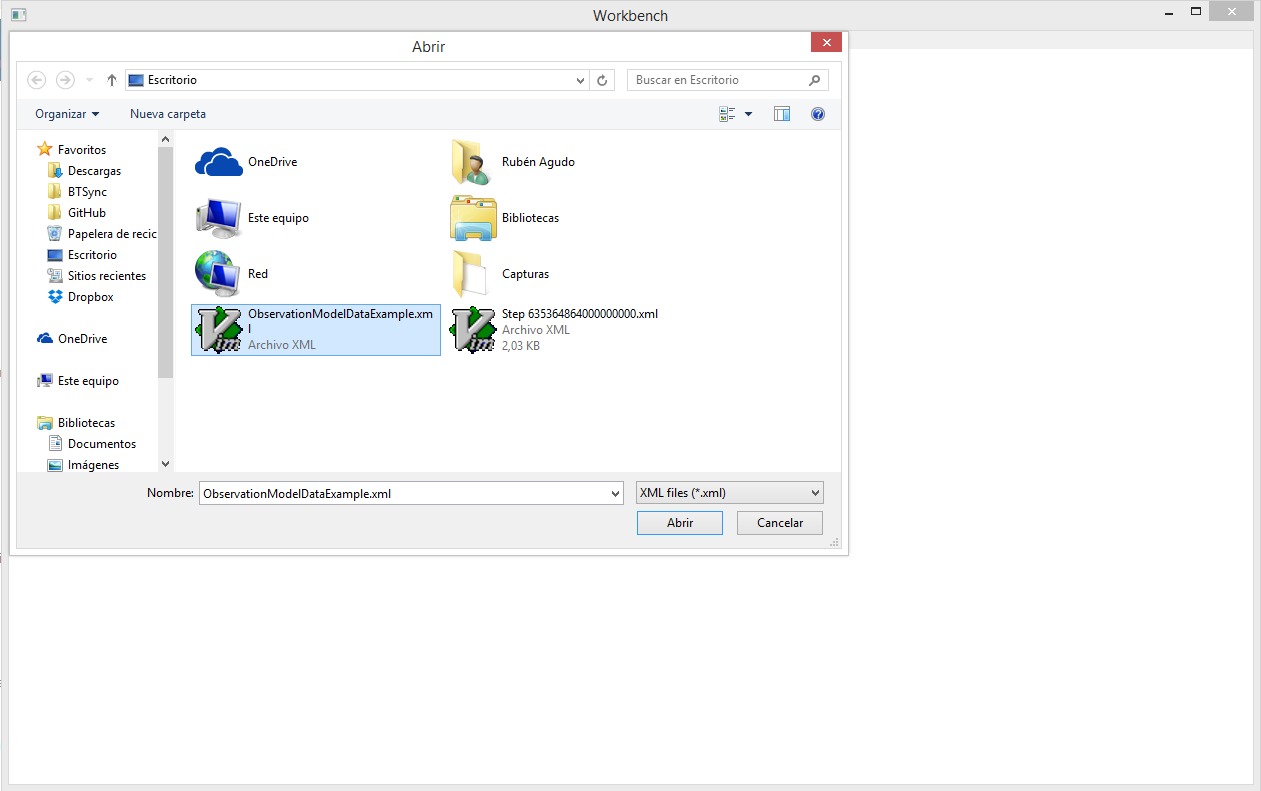
\includegraphics[width=0.75\linewidth]{./Figures/Capturas/AbrirXML1.PNG}
\caption{Abrir XML 1}
\label{fig:AbrirXML1}
\end{figure}

\begin{figure}[h]
\centering
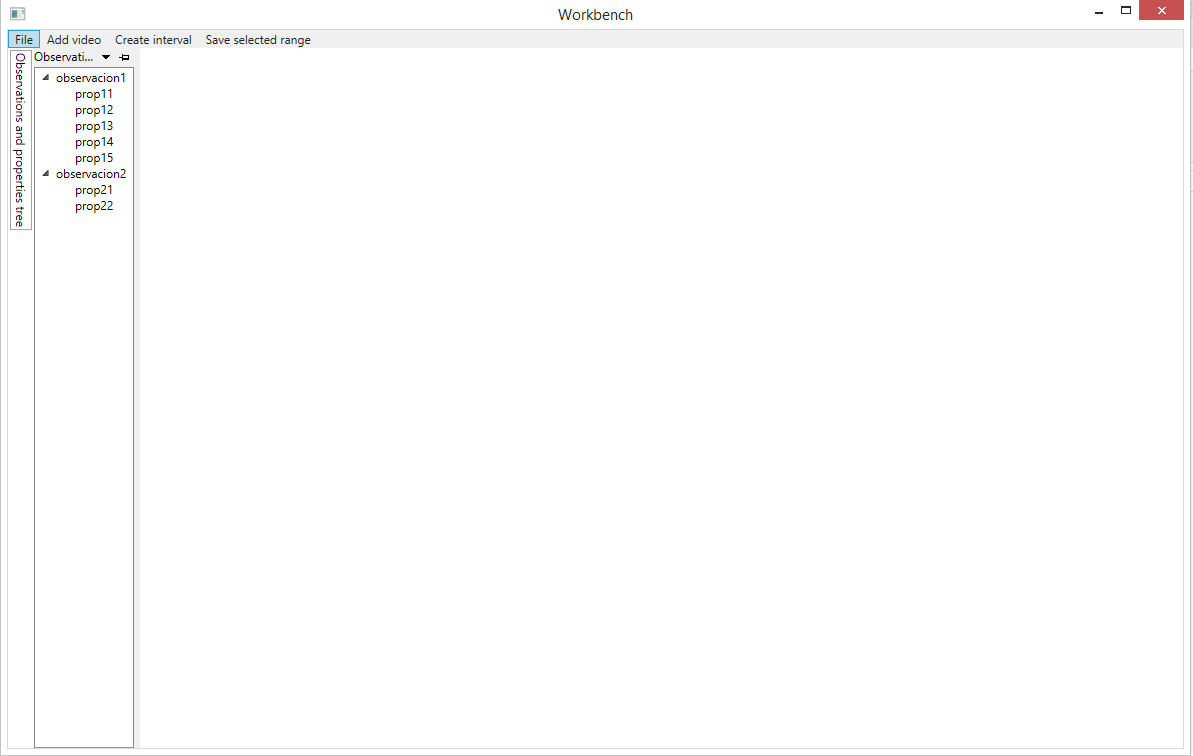
\includegraphics[width=0.75\linewidth]{./Figures/Capturas/AbrirXML2.PNG}
\caption{Abrir XML 2}
\label{fig:AbrirXML2}
\end{figure}

\begin{figure}[h]
\centering
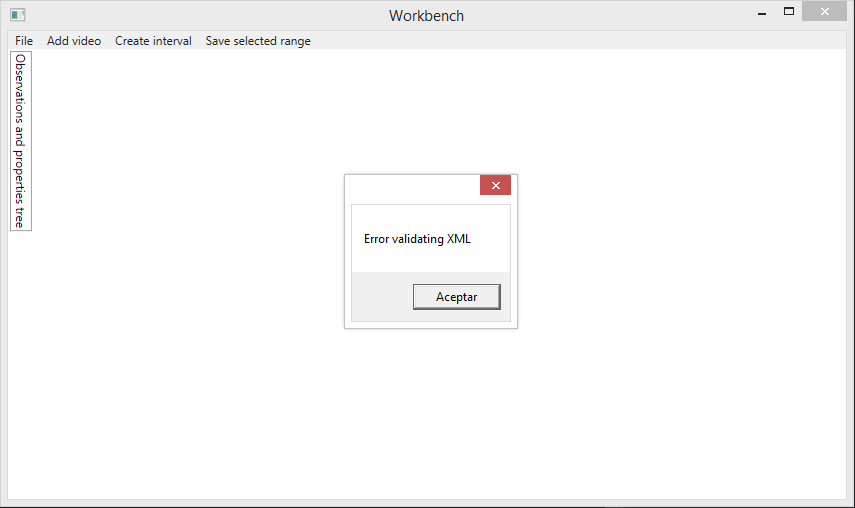
\includegraphics[width=0.9\linewidth]{./Figures/Capturas/AbrirXML3.PNG}
\caption{Abrir XML 3}
\label{fig:AbrirXML3}
\end{figure}

\begin{figure}[h]
\centering
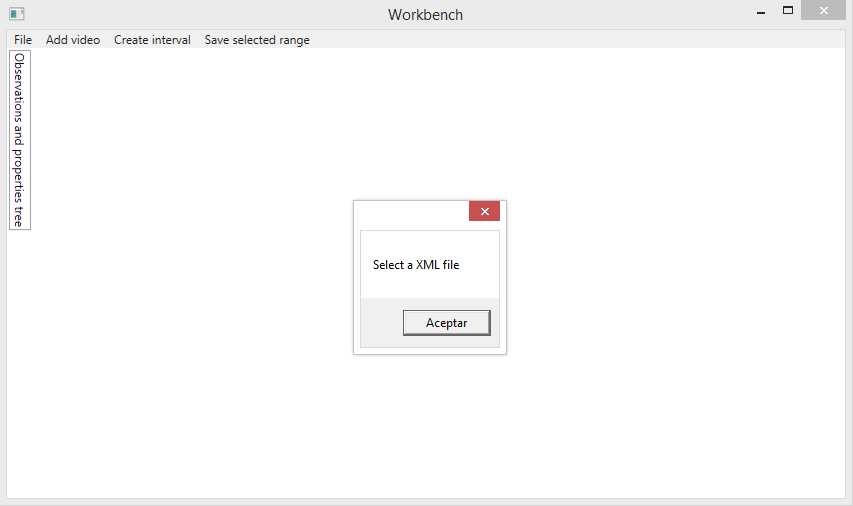
\includegraphics[width=0.9\linewidth]{./Figures/Capturas/AbrirXML4.PNG}
\caption{Abrir XML 4}
\label{fig:AbrirXML4}
\end{figure}

\begin{figure}[h]
\centering
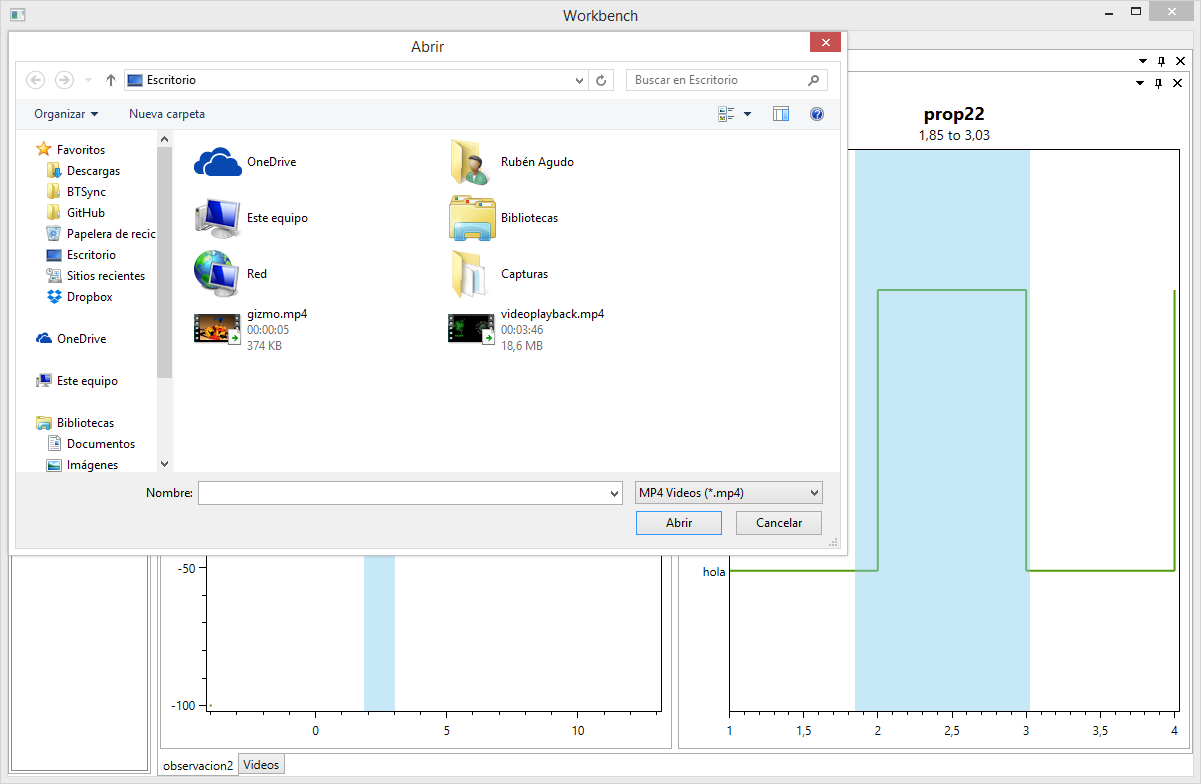
\includegraphics[width=0.9\linewidth]{./Figures/Capturas/CargarVideo.PNG}
\caption{Cargar V\'ideo}
\label{fig:CargarVideo}
\end{figure}

\begin{figure}[h]
\centering
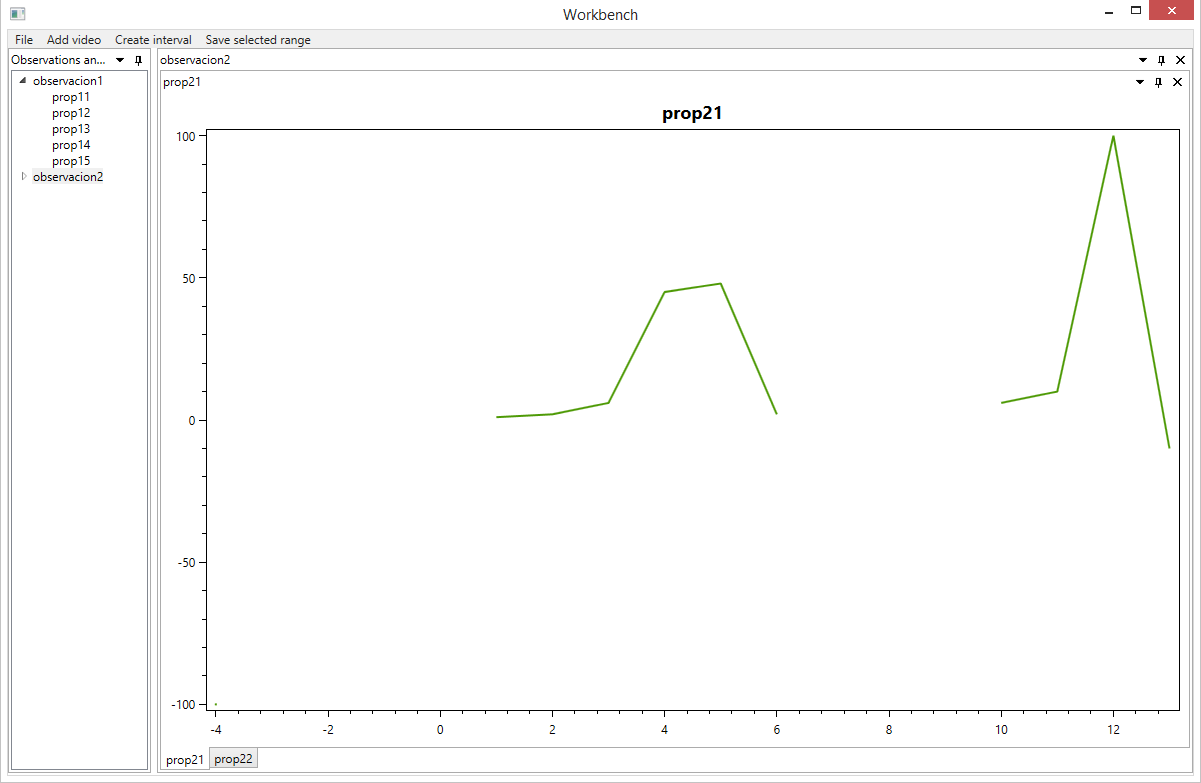
\includegraphics[width=0.9\linewidth]{./Figures/Capturas/CargarObservacionPropiedad.PNG}
\caption{Cargar Observaci\'on o Propiedad}
\label{fig:CargarObservacionPropiedad}
\end{figure}

\begin{figure}[h]
\centering
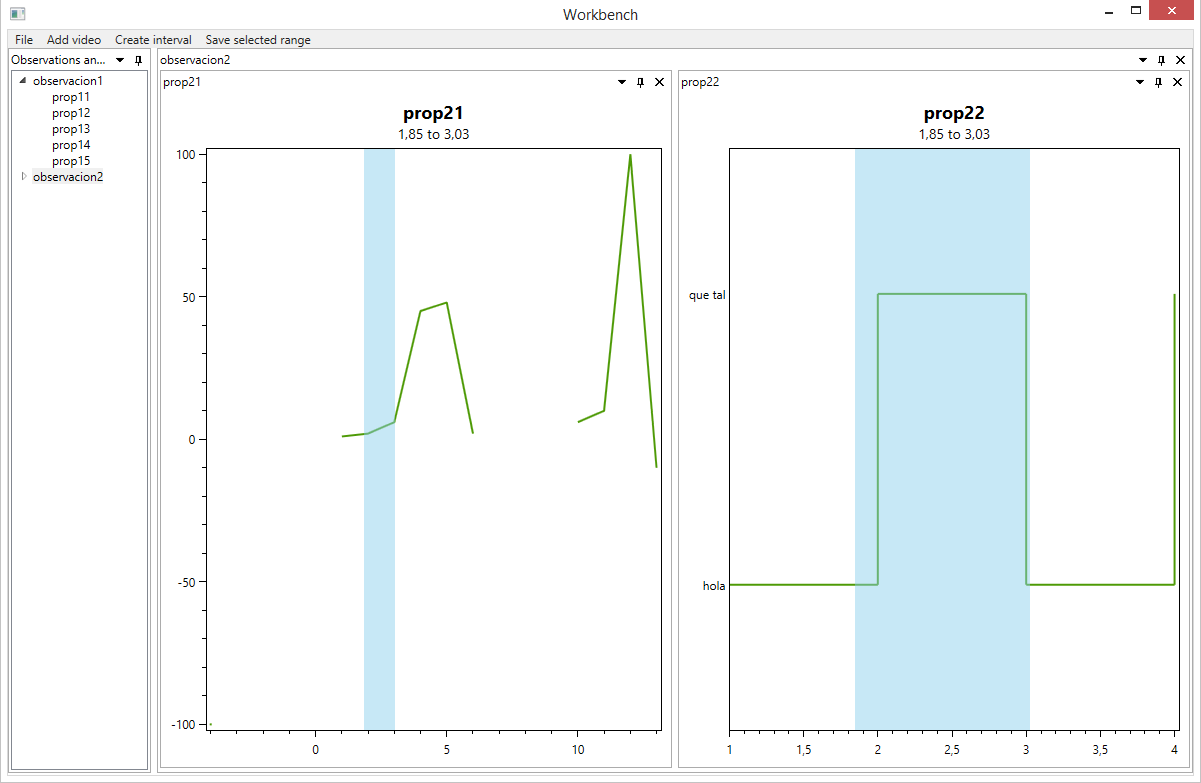
\includegraphics[width=0.9\linewidth]{./Figures/Capturas/SeleccionRango.PNG}
\caption{Seleccionar rango}
\label{fig:SeleccionarRango}
\end{figure}

\begin{figure}[h]
\centering
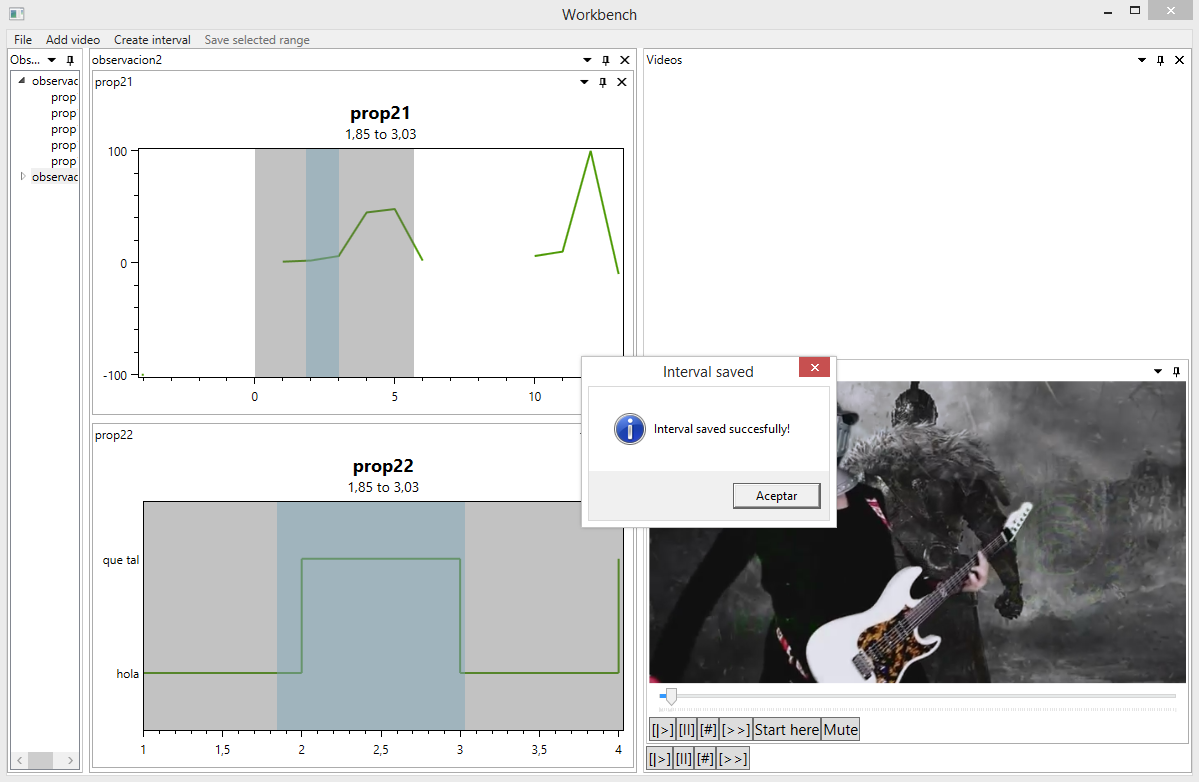
\includegraphics[width=0.9\linewidth]{./Figures/Capturas/IntervaloCreado.PNG}
\caption{Crear intervalo}
\label{fig:CrearIntervalo}
\end{figure}

\begin{figure}[h]
\centering
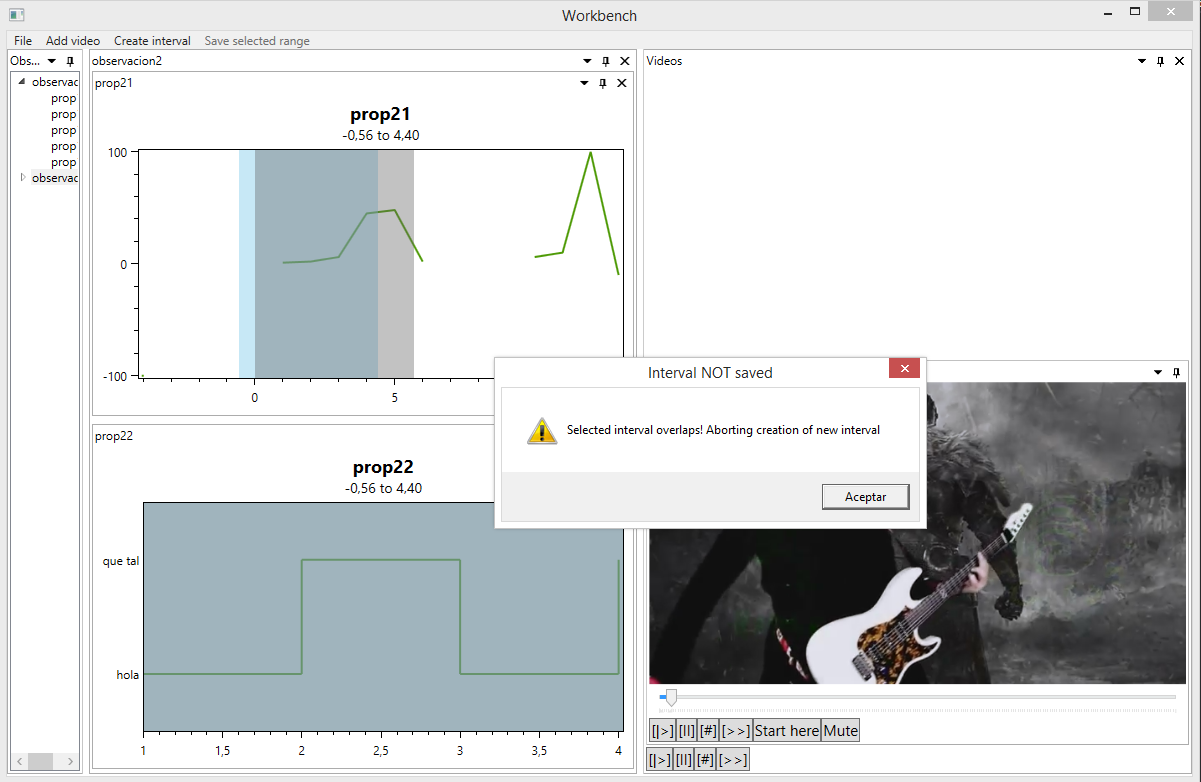
\includegraphics[width=0.9\linewidth]{./Figures/Capturas/IntervaloCreadoError.PNG}
\caption{Crear intervalo con  error}
\label{fig:CrearIntervaloError}
\end{figure}

\begin{figure}[h]
\centering
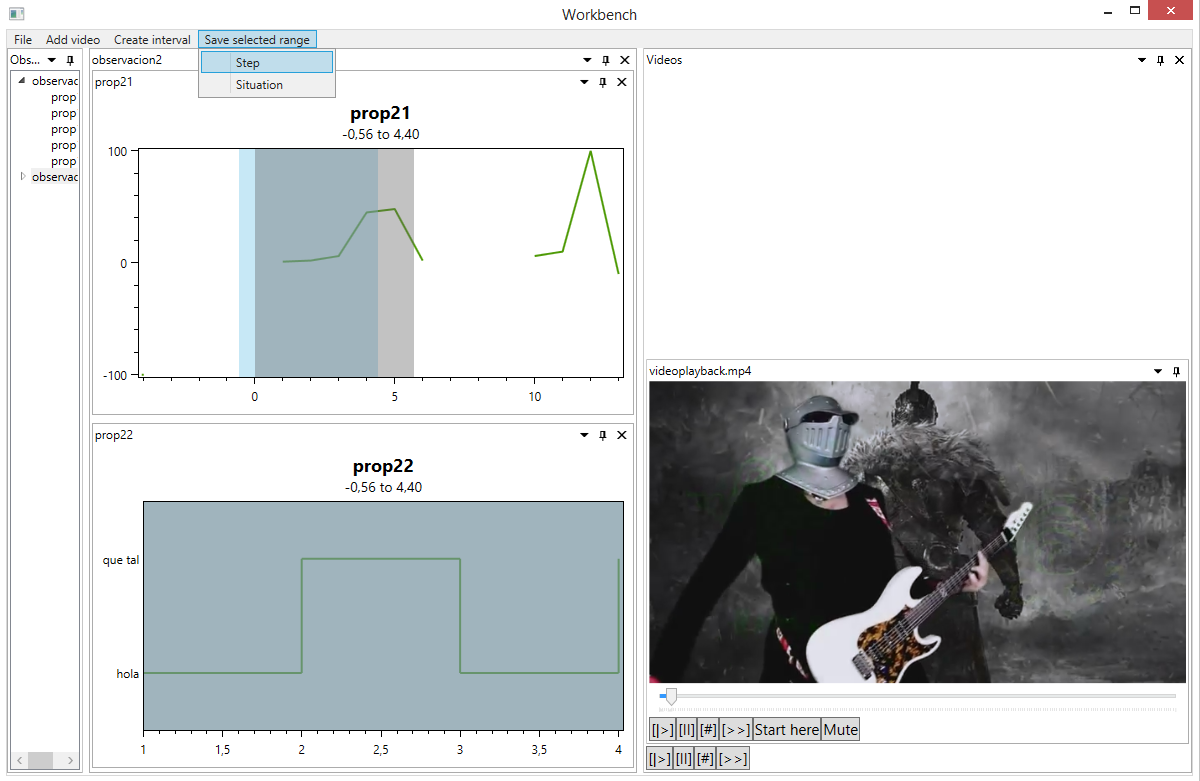
\includegraphics[width=0.9\linewidth]{./Figures/Capturas/GuardarPaso1.png}
\caption{Guardar paso 1}
\label{fig:GuardarPaso1}
\end{figure}

\begin{figure}[h]
\centering
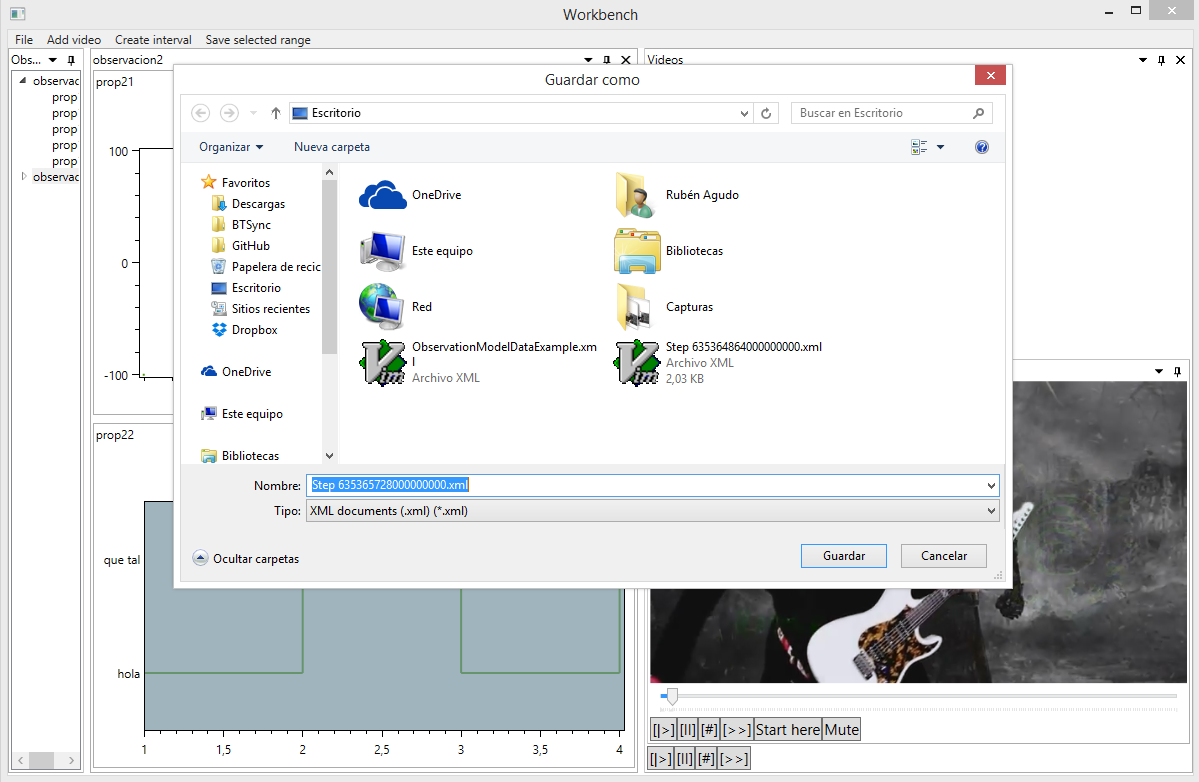
\includegraphics[width=0.9\linewidth]{./Figures/Capturas/GuardarPaso2.PNG}
\caption{Guardar paso 2}
\label{fig:GuardarPaso2}
\end{figure}

\begin{figure}[h]
\centering
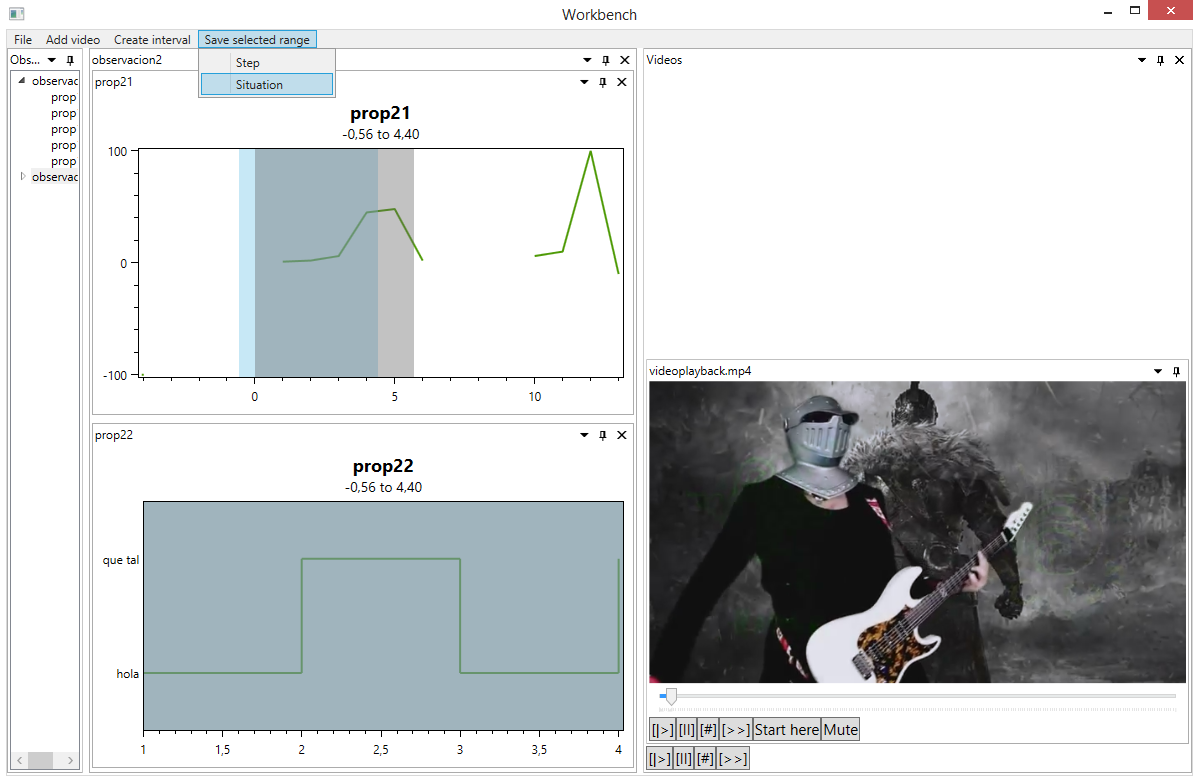
\includegraphics[width=0.9\linewidth]{./Figures/Capturas/GuardarSituacion1.png}
\caption{Guardar situaci\'on 1}
\label{fig:GuardarSituacion1}
\end{figure}

\begin{figure}[h]
\centering
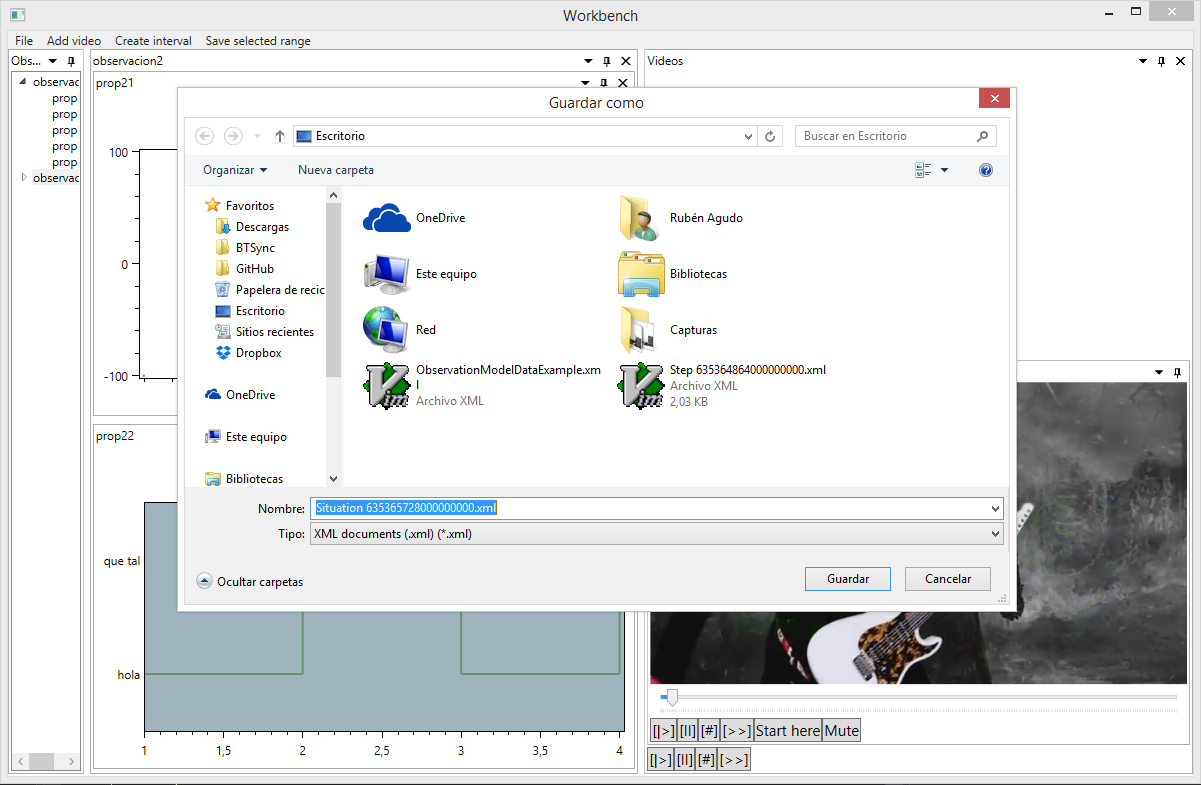
\includegraphics[width=0.9\linewidth]{./Figures/Capturas/GuardarSituacion2.PNG}
\caption{Guardar situaci\'on}
\label{fig:GuardarSituacion2}
\end{figure}
